
\chapter{Lecture 7: Special functions (and some revision)} \label{lec7}

\subsection{Index laws} \label{base} \label{index} \label{exponent}
The index laws are a set of algebraic rules for handling \textbf{indexes}; they are a completely indispensible tool for anybody who wants to do even basic mathematics. You may already know some (or all) of these laws, and you have (possibly without realising it) been using them already in this subject. \\

\noindent Index laws tell us how to manipulate expressions of the form $b^x$. We call $b$ the \textbf{base}, and we call $x$ the \textbf{index}, or \textbf{exponent.} We say ``$b$ to the $x$.'' By convention, \textbf{$\boldsymbol{b}$ is a real valued constant such that $\boldsymbol{b \geq 0,}$} (see section \ref{fractional indices} for an explanation of why this must be so) and $x$ is a real number. \\

\noindent Indexes tell us how many times to multiply the base by itself. For example, the expression $3^2$ has base $3$ and index $2$; it asks us to multiply $3$ by itself twice (giving 9). \\

\noindent Some numbers can be thought of as having indexes even though we might not write the indexes explicitly. For example, when we write the number $2$, we could just as correctly write $2^1$, because $2^1 = 2$. We have already used one of the most important index laws; in sections \ref{sec416} and \ref{secbinom}, we mentioned that $a^0 = 1$, for any real number $a$.
Before we look at another example where we have already used index laws, let's list all of the index laws themselves. \\

\textbf{Index laws:}
\begin{itemize}
\item $b^xb^y = b^{x+y}$ \hfill  (I1) \smallskip \smallskip
\item $(b^x)^y = b^{xy}$ \hfill  (I2) \smallskip \smallskip
\item $b^0 = 1$ \hfill  (I3)
\item $\displaystyle{b^{-x} = \frac{1}{b^x} = \brac{\frac{1}{b}}^x}$ \hfill  (I4)
\item $(ab)^x = a^xb^x$   \hfill  (I5)
\end{itemize}
Notice that law (I1) applies when we have the same base, while law (I5) applies when we have the same index. \\

\subsection{Example}

We have implicitly used at least one index law when we have cancelled common factors from fractions. For example,
\begin{align*}
\frac{(1-p)b}{b} & = (1-p)\frac{b^1}{b^1} \\
		   & = (1-p)b^{1}b^{-1}  \tag{since $\frac{1}{b^y} = b^{-y}$, law (I4)} \\
		   & = (1-p)b^{1-1} \tag{since $b^xb^y = b^{x+y}$, law (I1)} \\
		   & = (1-p)b^0 \\ 
		   & = (1-p). \tag{since $b^0 = 1$, law (I3)}
\end{align*}

%\noindent By convention, the index laws assume that the base, $b$, is a positive real number. If we want to use the laws on a negative number then we can write $-b$, where $b$ is the positive part. The exponent can be any real number. \\

\subsection{Example}
Notice how laws (I4) and (I1) tell us how to simplify complicated fractions with many exponents; for example,
\begin{align*}
\frac{a^5b^xb^y}{b^{x+y}a^4} & = a^{5-4}\frac{b^xb^y}{b^{x+y}} \tag{since $\frac{a^5}{a^4} = a^{5-4}$, by laws (I4) and (I1)} \\
						       & = a^1 \frac{b^{x+y}}{b^{x+y}} \tag{since $b^xb^y = b^{x+y}$, by law (I1)} \\
						       & = ab^{(x+y)-(x+y)} \tag{by laws (I4) and (I1) again} \\
						       & = ab^0 \\
						       & = a. \tag{as $b^0 = 1$ by law (I3)}
\end{align*}


\subsection{Example}
Try to complete the following yourself, then look at the solutions below.
\begin{enumerate}
\item Write the following using index notation: \\
(i) \;\; $3\times3\times3\times3$, \qquad (ii) \;\; $2\times2^4$, \qquad (iii) \;\;$(5\times5)^6$.

\item Simplify the following using index notation: \\
(i) \;\; $5^4\times5^{-2}\times3^3$, \qquad (ii)\;\; $3^2\times2^4,$ \qquad (iii) \;\;$\frac{2\times2\times2}{2^4}$.

\item Are the following statements true or false? If false, write the correct right hand side: \\
(i)\;\; $4^2 \times 2^5 = 8^3$, \qquad (ii) \;\; $\frac{3^2}{7^2} = \bfrac{3}{7}^2$ \qquad (iii) \;\; $(4^2)^3 = 12^3$
\end{enumerate}

\vspace{1.5cm}
\noindent \textit{Solutions:}
\begin{enumerate}
\item Written using index notation:
\begin{align*}
\text{(i)} & \;\; 3\times3\times3\times3 = 3^{1+1+1+1} = 3^4 \tag{using (I1)} \\
\text{(ii)} & \;\; 2\times2^4 = 2^{1+4} = 2^5 \tag{using (I1)} \\
\text{(iii)} & \;\; (5\times5)^6 = 5^6\times5^6 = 5^{6+6} = 5^{12} \tag{using (I5) and (I1)}.
\end{align*}
\item Simplified using index notation:
\begin{align*}
\text{(i)} & \;\; 5^4\times5^{-2}\times3^3 = 5^{4-2}\times3^3 = 5^2\times3^3 \tag{using (I1)} \\
\text{(ii)} & \;\; 3^2\times2^4 \tag{we can't do anything} \\
\text{(iii)} & \;\; \frac{2\times2\times2}{2^4} = \frac{2^3}{2^4} = 2^{3-4} = 2^{-1} = \frac{1}{2} \tag{using (I1) and (I4)}
\end{align*}
\item We have:
\begin{align*}
\text{(i)} & \;\; 4^2 \times 2^5 = (2^2)^2 \times 2^5 = 2^{2\times2}\times2^5 = 2^{4+5} = 2^9 = 2^{3\times3} = \brac{2^3}^3 = 8^3 \tag{True} \\
\text{(ii)} & \;\; \frac{3^2}{7^2} = \bfrac{3}{7}^2 \tag{True by rule (I5), with $a=3$ and $b = \frac{1}{7}$} \\
\text{(iii)} & \;\; (4^2)^3 = 16^3 \neq 12^3 \tag{False}
\end{align*}
\end{enumerate}

\subsection{Fractional indices and roots} \label{fractional indices}
When we introduced the index laws in the previous section, why did we use the convention that $b$ must be a real number greater than or equal to zero? To answer this question we need to understand what fractional indices mean. \\ \label{inverse operation}

\noindent You may already know that the square root of a number, $b$, is the number, $t$, which multiplied by itself gives $b$. For example, $2^2 = 4,$ so $2$ is the square root of $4$; or $3^2 = 9,$ so $3 = \sqrt{9}$. In other words, the square root of $b$ is the number, $t$, which satisfies the equation
\[
t^2 = b.
\]
We write, $t = \sqrt{b}$. Similarly, we can define the cube root of $b$, to be the number, $k$, which satisfies the equation
\[
k^3 = b
\]
We write $k = \sqrt[3]{b}$, and say ``$k$ is the cube root of $b$.'' For example, $2^3 = 8$, so $2 = \sqrt[3]{8}$. Also, $3^3 = 27$, so $3 = \sqrt[3]{27}$. We can do this for any natural number, $n$; we define:

\bigskip
\hfil\fbox{
\begin{minipage}{0.5\columnwidth}{

\vskip 0.04cm
\begin{center}
the $n^{\text{th}}$ root of $b$ is the number, $y$, that satisfies the equation \\ $y^n = b$
\end{center}
}
\end{minipage}}
\bigskip

\noindent We write $y = \sqrt[n]{b},$ and we say ``$y$ is the $n^{\text{th}}$ root of $b$.'' Now, we are going to use this definition to prove that $b^{\frac{1}{2}} = \sqrt{b}$, and that $b^\frac{1}{3} = \sqrt[3]{b}$, and more generally, that $b^\frac{1}{n} = \sqrt[n]{b}$. This is a very important result! It means that we can drop the symbol, $\sqrt[n]{\phantom{2}}$, and just use indices to represent roots. \\

\noindent The proof is simple, it only uses index law (I2). We want to show that
\[
y^n = b \;\;\; \text{implies} \;\;\; y = b^\frac{1}{n}.
\]
Raising both sides of $y^n = b$ to the power of $\frac{1}{n}$ gives
\[
\brac{y^n}^\frac{1}{n} = b^\frac{1}{n}.
\]
Using index law (I2) gives
\[
y^{n\times\frac{1}{n}} = b^\frac{1}{n}.
\]
Simplifying the left hand side gives
\[
y = b^\frac{1}{n}.
\]
Now, recall that our definition of $n^{\text{th}}$ root also implies that $y = \sqrt[n]{b}$. Hence,
\[
y = \sqrt[n]{b}, \qquad \text{and} \qquad y = b^\frac{1}{n}.
\]
So, $\sqrt[n]{b} = b^\frac{1}{n}$. We can now, for all intents and purposes, if we wish, stop using the $\sqrt{\phantom{n}}$ symbol, and just use indices. Furthermore, whenever we have a problem involving roots, we can represent the roots as indices, and then use the index laws to help us solve the problem. \\

\noindent Before we get onto an example, we are now set up to understand why it was stated that the base, $b$, must satisfy $b \geq 0$, when we introduced the index laws. What happens if we take $b = -1$, and $n = 2$ in the equation $y^n = b$? We are looking for the solution, $y$, to the equation,
\[
y^2 = -1
\]
This is impossible to do with real numbers; there is no real number that, when squared, gives a negative number. Multiplying a real number by itself always yields a positive number. This implies that the number $\sqrt{-1}$ is not a real number. So, if we did not define $b$ to be necessarily positive, then we would end up having to deal with expressions of the form
\[
(-1)^\frac{1}{2} = \sqrt{-1}.
\]
Dealing with such expressions can be achieved using a set of numbers (and some associated mathematical rules) called the complex numbers. However, we won't be dealing with complex numbers in this subject.

\subsubsection{Example}
Let $x$ be a positive real number. Simplify the expression,
\[
\frac{\sqrt{x^3}}{x^\frac{3}{2}}
\]
Rewriting the square root as an index gives
\[
\frac{\sqrt{x^3}}{x^\frac{3}{2}} = \frac{\brac{x^3}^\frac{1}{2}}{x^\frac{3}{2}}.
\]
Using index law (I2) gives
\[
\frac{\brac{x^3}^\frac{1}{2}}{x^\frac{3}{2}} = \frac{x^{3\times\frac{1}{2}}}{x^\frac{3}{2}}.
\]
Simplifying the expression on the right hand side gives,
\[
\frac{x^{3\times\frac{1}{2}}}{x^\frac{3}{2}} = \frac{x^\frac{3}{2}}{x^\frac{3}{2}} = 1.
\]
Hence $\frac{\sqrt{x^3}}{x^\frac{3}{2}} = 1$.
%Another way to think of this is that the square root is \textit{defined as} the \textbf{inverse operation} to taking the square of a number; that is, taking the square root ``undoes'' the operation of taking the square. For example, taking the square root of both sides of the above expression gives,
%\[
%\sqrt{y^2} = \sqrt{b}.
%\]  
%So, we can see that, by our definition of square root, we must have $\sqrt{y^2} = y$.
%\[
%\sqrt{2^2} = \sqrt{4}
%\]
%So, since the square root is inverse to the square operation, we can simplify the expression on the left hand side by letting, $\sqrt{2^2} = 2$. Hence we discover that
%\[
%2 = \sqrt{4}.
%\]




\subsection{Introduction to functions and their graphs}
We already introduced functions in some detail in section \ref{sectionfunctions}. If you have not already read this section, then go back and do it now. \\

\noindent The most compact way to define a function is using an equation as a rule. \\
For example:
\[
f(x) = x - 2
\]
Which can be read as, ``the value of the function $f$, for any input numbe $x$, is $x-2$.'' \\

\noindent One way to picture what a function does is to draw part of its \textbf{graph} on a \textbf{cartesian coordinate system} (that is, on $x,y$-axes).  \label{cartesian coordinate system} \label{graph}
\begin{center}
	\begin{tikzpicture}
	\draw [fill = black] (0,0) circle (0.05cm) node [below left] {$(0,0)$};
	\draw [dashed] (1,1.3) -- (1,-0.1) node [below] {$x_1$};
	\draw [dashed] (1,1.3) -- (-0.1,1.3) node [left] {$y_1$};
	\draw [->] (-0.2,0) -- (3,0) node [below right] {$x$};
	\draw [->] (0,-0.2) -- (0,2.8) node [above left] {$y$};
	\draw [fill = black] (1,1.3) circle (0.05cm) node [above right] {$(x_1,y_1)$};
	\end{tikzpicture}
\end{center}
The figure above depicts a cartesian coordinate system. The $x$ and $y$ axes are number lines (see the diagrams of number lines in section \ref{number line} on page \pageref{number line}). We can mark any point on the diagram, given the point's coordinates, $(x_1,y_1)$; where $x_1$ is the distance from $(0,0)$ at which the point lies, in the $x$-direction, and $y_1$ is the distance from $(0,0)$ at which the point lies, in the $y$-direction. We call the point, $(0,0),$ the \textbf{origin}. When we draw a graph, we usually draw the $x$ and $y$ axes so that they intersect eachother at the origin. \\

\noindent The graph of a function consists of points $(x,f(x))$. So, to find the points, $(x,y)$, on a cartesian coordinate system, we let $y = f(x)$. 

\subsection{Straight line functions [$y = mx + c$]} \label{secline}
Consider the function $f(x) = -2x + 4$. This is an example of a function that is linear. The graph of this function is a straight line. Straight line functions are of the form $f(x) = mx + c$, where $m$ and $c$ are constants (fixed real numbers). In this case we have $m = -2$ and $c = 4$. To graph it, we let $y = f(x)$. That is, we let $y = mx+c$; then we plot the points $(x,y),$ i.e., the points $(x,mx+c).$ \\

\noindent In order to plot a straight line, we only need to calculate two points manually, then we just draw a line passing through both those points. We can choose which two points are easiest to calculate manually; usually, the points corresponding to $x = 0$ and $x = 1$ are easiest. We have,
\[
x = 0 \;\; \text{gives the point:} \;\; (x,y) = (0,-2\times0 + 4) = (0,4), \tag{f(0) = 4}
\]
and
\[
x = 1\;\; \text{gives the point:} \;\; (x,y) = (1,-2\times1+4) = (1,2). \tag{f(1) = 2}
\]
Plotting these two points we get
\begin{center}
	\begin{tikzpicture} [scale = 0.7]
	\draw [fill = black] (0,0) circle (0.05cm) node [below left] {$(0,0)$};
	\draw [dashed] (1,2) -- (1,-0.1) node [below] {$1$};
	\draw [dashed] (1,2) -- (-0.1,2) node [left] {$2$};
	\draw [->] (-1,0) -- (5,0) node [below right] {$x$};
	\draw [->] (0,-1) -- (0,5.5) node [above left] {$y$};
	\draw [fill = black] (1,2) circle (0.08cm) node [above right] {$(1,f(1))$};
	\draw [fill = black] (0,4) circle (0.08cm) node [above right] {$(0,f(0))$} node [left] {$4$};
	\end{tikzpicture}
\end{center}
Drawing a line through both these points gives us the graph of $f(x),$
\begin{center}
	\begin{tikzpicture} [scale = 0.7]
	\draw (6,5) node {Graph of $f(x) = -2x + 4$.};
	\draw [fill = black] (0,0) circle (0.05cm) node [below left] {$(0,0)$};
	%\draw [dashed] (1,2) -- (1,-0.1) node [below] {$1$};
	%\draw [dashed] (1,2) -- (-0.1,2) node [left] {$2$};
	\draw [->] (-1,0) -- (5,0) node [below right] {$x$};
	\draw (3,-2) -- (-1,6) node [above left] {$f(x)$};
	\draw [->] (0,-1) -- (0,5.5) node [above left] {$y$};
	\draw [fill = black] (1,2) circle (0.08cm) node [above right] {$(1,2)$};
	\draw [fill = black] (0,4) circle (0.08cm) node [above right] {$(0,4)$};
	\end{tikzpicture}
\end{center}
Notice that the function crosses (intercepts) the $y$ axis at $y = 4$. In general, for a straight line of the form $f(x) = mx + c$, the constant $c$ represents the point on the $y$-axis that the line will touch (this point is called the \textbf{$\mathbf{y}$-intercept}). \label{y-intercept}

%DID NOT INTRODUCE m BECAUSE INTERESTING IN CALCULUS.

\section{Continuity and discontinuity} \label{continuity and discontinuity}
\noindent For a function to be \textbf{continuous} means, intuitively, that we can draw it without lifting our pen off the page. Straight line functions of the form $f(x) = mx+c$ are all continuous. We will see many more examples of continous functions in the next few sections. Formally, a function is continuous if
\[
\lim_{x \rightarrow a}f(x) = f(a), \qquad \text{for all points, $a$, in the domain of the function.}
\]

\noindent However, some functions that we will see (particularly rational functions) are \textbf{discontinuous}. They have points in their domain for which the function is undefined. It is not possible to draw them without lifting your pen off the page. A very ubiquitous example is the function $f(x) = \frac{1}{x}$ (we will soon see that this is a rational function). This function is discontinuous at $x = 0$ because when $x = 0$ the expression $\frac{1}{x}$ is undefined.   \\

\noindent For examples of continuous and discontinuous functions, look at all of the graphs within sections \ref{powers (natural number)} to \ref{exponentials}. If any of the functions pictured are discontinuous we will explicitly state this, otherwise they are all continuous.


\section{Non-linear functions} \label{continuous functions} \label{discontinuous functions}
Non-linear functions have graphs that are not straight lines. In this section we will introduce various types of functions, including \textbf{powers (natural number)},  \textbf{polynomials}, \textbf{rational functions}, \textbf{powers (non-integer)}, and \textbf{exponentials}. Most variations of these types of functions, as we will see, are not straight lines. \\


\subsection{Powers (natural number) [$y = x^n$]} \label{powers (natural number)}
Power functions are of the form $f(x) = x^m$ for some real number $m$. When $m$ is a natural number greater than 1 (i.e., a positive whole number greater than 1), the graphs of these functions can be characterised by whether $m$ is even or $m$ is odd. \\

\noindent When $m$ is even the function is bowl shaped (see diagram below). This shape is sometimes referred to as `concave up' or `convex.' \\

\noindent As you can see from the graphs below, there are two basic shapes (one for even $m$ and one for odd $m$). The graphs maintain the same basic shape as the power, $m$, increases; the only feature that changes as the powers increase is that the graphs become flatter near the $x$-axis, and they become steeper (they rise or fall more quickly for increasing or decreasing $x$).

\begin{center}
	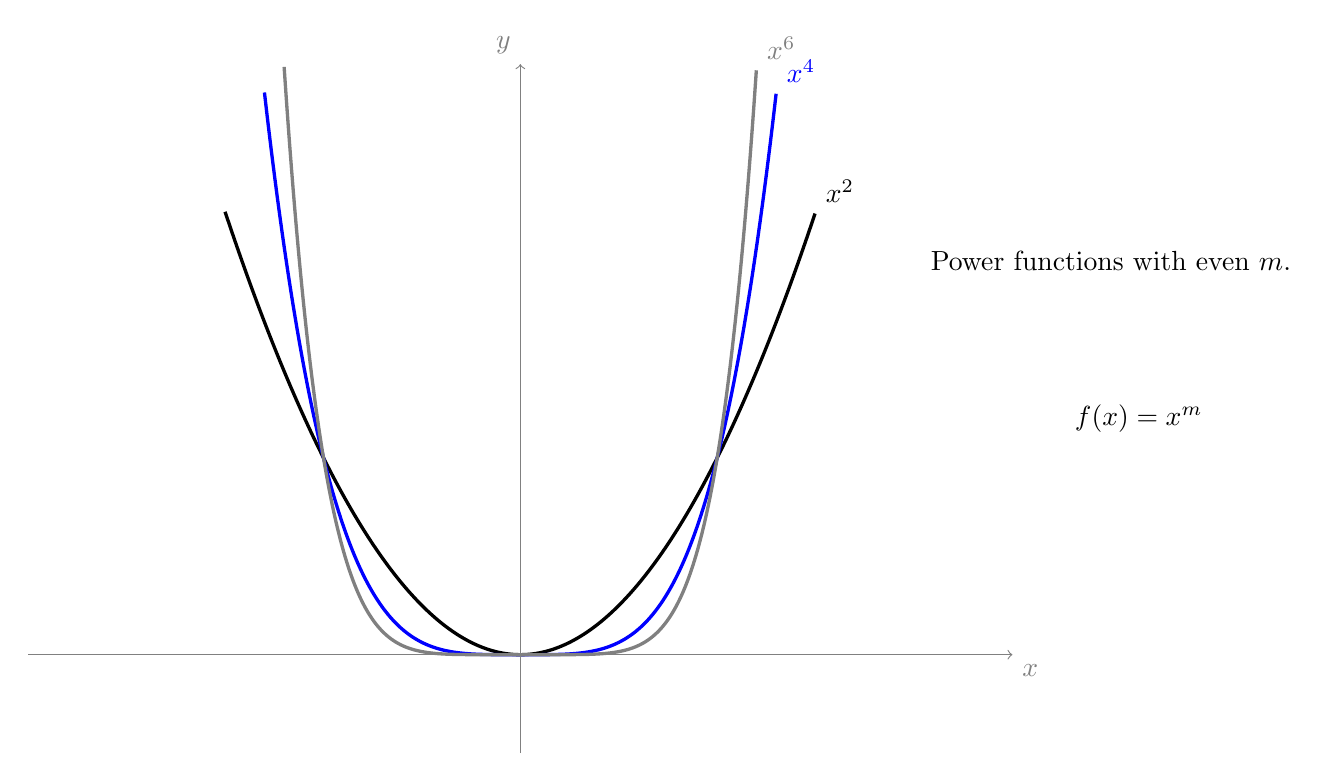
\begin{tikzpicture} [scale = 2.5]
	\draw[very thick, domain = -1.5:1.5, samples=200, smooth] plot (\x, {\x*\x}) node [above right] {$x^2$};
	\draw[very thick, blue, domain = -1.3:1.3, samples=200, smooth] plot (\x, {\x*\x*\x*\x}) node [above right] {$x^4$};
	\draw[very thick, gray, domain = -1.2:1.2, samples=200, smooth] plot (\x, {\x*\x*\x*\x*\x*\x}) node [above right] {$x^6$};
	\draw [gray, ->] (0,-0.5) -- (0,3) node [above left] {$y$};
	\draw [gray, ->] (-2.5,0) -- (2.5,0) node [below right] {$x$};
	\node [fill = white] at (pi,1.2) {$f(x) = x^m$};
	\draw (3,2) node {Power functions with even $m$.};
	\end{tikzpicture}
\end{center}

\begin{center}
	\begin{tikzpicture} [scale = 2]
	\draw[very thick, domain = -1.3:1.3, samples=200, smooth] plot (\x, {\x*\x*\x}) node [above right] {$x^3$};
	\draw[very thick, blue, domain = -1.2:1.2, samples=200, smooth] plot (\x, {\x*\x*\x*\x*\x}) node [above right] {$x^5$};
	\draw[very thick, gray, domain = -1.16:1.16, samples=200, smooth] plot (\x, {\x*\x*\x*\x*\x*\x*\x}) node [above right] {$x^7$};
	\draw [gray, ->] (0,-2.4) -- (0,3) node [above left] {$y$};
	\draw [gray, ->] (-2.5,0) -- (2.5,0) node [below right] {$x$};
	\draw (3,2) node {Power functions with odd $m$.};
	\node [fill = white] at (pi,1.2) {$f(x) = x^m$};
	\end{tikzpicture}
\end{center}

\subsection{Polynomials [$y = a + bx + cx^2 + \ldots$]} \label{polynomials}
The term ``''polynomial,'' similar to the term, ``binomial,'' can be broken down into two parts: ``poly'' (meaning ``many''); and ``nomial'' (meaning ``parts,'' or ``terms''). \\

\noindent Polynomials are functions of the form

	\bigskip
	
	\hfil\fbox{
	\begin{minipage}{0.45\columnwidth}{
	
	\vskip 0.04cm
	\begin{center}
	$f(x) = a + bx + cx^2 + dx^3 + \ldots + \alpha x^n.$
	\end{center}
	}
	\end{minipage}}
	\bigskip
	
\noindent Where $a,b,c,\ldots,\alpha$ are real valued constants (any or all of which can be equal to zero). Consider the polynomial, $k(x)$, which has the following values for its constants:
\[
c = 1 \;\; (\text{and} \; a,b,d,\ldots,\alpha \; \text{all equal $0$}).
\]
We get
\begin{align*}
k(x) & = 0 + 0\times x + 1\times x^2 + 0\times x^3 + \ldots+ 0 \times x^n \\
       & = x^2.
\end{align*}
So $k(x) = x^2$; but $x^2$ is a power function (see section \ref{powers (natural number)}). Indeed, power functions are just special cases of polynomials (or we could say that polynomials are built out of power functions). \\

\noindent Now consider the polynomal, $q(x),$ which has all of its constants equal to zero except for $a,$ for which we set $a = 1$. For this polynomial we get,
\begin{align*}
q(x)  & = 1 + 0\times x + 0 \times x^2 + 0 \times x^3 + \ldots + 0\times x^n \\
	& = 1.
\end{align*}
So constants, like the number 1, are also polynomials! \\


\noindent  \textbf{When we add or multiply polynomials, we get a new polynomial}. For example, take the polynomials, $g(x)$ and $h(x)$, with $g(x) = 3x^2 + 4$ and $h(x) = x^3 + x^2 + 1$. Then 
\begin{align*}
g(x) + h(x) & = 3x^2 + 4 + x^3 + x^2 + 1  \\
		 & = x^3 + 4x^2 + 5. \tag{which is a polynomial} 
\end{align*}
Also,
\begin{align*}
g(x)h(x) & =  \brac{3x^2 + 4}\brac{x^3 + x^2 + 1} \\
	      & = 3x^2\brac{x^3 + x^2 + 1} + 4\brac{x^3 + x^2 + 1} \\
	      & = 3x^2x^3 + 3x^2x^2 + 3x^2 + 4x^3 + 4x^2 + 4 \\
	      & = 3x^{2+3} + 3x^{2+2} + 3x^2 + 4x^3 + 4x^2 + 4 \tag{using index law (I1)} \\
	      & = 3x^5 + 3x^4 + 4x^3 + 7x^2 + 4. \tag{which is a polynomial}
\end{align*}

\subsubsection{Some important properties of polynomials, when $x \in [0,1]$:}
Probabilities are real numbers that lie between $0$ and $1$. Since we are working with probabilities, it is worth taking a closer look at the behaviour of polynomials when their domain is the interval~$[0,1].$ \\

\noindent Consider the following graph of the polynomials, $x$, $x^2$, and $x^3$:
\begin{center}
	\begin{tikzpicture} [scale = 2.5]
	\draw[very thick, domain = 0:1.5, samples=200, smooth] plot (\x, {\x}) node [above right] {$x$};
	\draw[very thick, blue, domain = 0:1.4, samples=200, smooth] plot (\x, {\x*\x}) node [above right] {$x^2$};
	\draw[very thick, gray, domain = 0:1.36, samples=200, smooth] plot (\x, {\x*\x*\x}) node [above right] {$x^3$};
	\draw [gray, ->] (0,-0.5) -- (0,2.7) node [above left] {$y$};
	\draw [gray, ->] (-0.5,0) -- (2.5,0) node [below right] {$x$};
	\draw (3,2) node {Polynomials: $x,x^2,x^3$.};
	\node [fill = white] at (pi,1.2) {$h(x) = x^m$};
	\draw [dashed] (1,1) -- (-0.1,1) node [left] {$1$};
	\draw [dashed] (1,1) -- (1,-0.1) node [below] {$1$};
	\end{tikzpicture}
\end{center}
What difference do you notice about the comparative values of these functions on the interval $x \in [0,1]$, versus the interval $x > 1$? Consider what happens when we square a number between 0 and 1. For example,
\begin{align*}
\brac{\frac{1}{2}}^2 & = \frac{1^2}{2^2} \tag{index law (I5)} \\
				   & =  \frac{1}{4}.
\end{align*}
When we square a number, say $b$, between 0 and 1, we always get a number less than $b$ (or equal to $b$ in the case that $b$ is actually equal to 0 or 1). In contrast, when we square a number greater than~1, say $d$, we always get a number greater than $d$. In fact, the same goes for any natural number power of $x$; this fact is reflected in the above graph of the polynomials $x, x^2, x^3$. \\

\noindent This feature of the graphs of polynomials is important to remember, since we will mostly be dealing with probabilities; taking natural number powers of variables representing our probabilities will lead to lesser (or at most equal) values. \\

\noindent Another important fact to remember is that \textbf{products and powers of numbers in~$\boldsymbol{[0,1]}$ stay in $\boldsymbol{[0,1]}$}. This fact can also be demonstrated effectively using graphs. We will illustrate with the following examples. \\

\noindent Firstly however, note that if $x \in [0,1]$, then $(1-x) \in [0,1].$ To see this, let $x \in [0,1]$. Then $0 \leq x \leq 1$. Subtracting 1 from all sides (Rule (1) for rearranging inequalities, see section \ref{secinecrule}) gives $-1 \leq x-1 \leq 0$. Then, multiplying all sides by $-1$ (Rule (3) for rearranging inequalities) gives $1 \geq 1 - x \geq 0$, which is the interval $[0,1]$. So, $(1-x) \in [0,1].$ Hence, if $x \in [0,1]$ then $(1-x) \in [0,1],$ as required. \\

\noindent Now, consider the expressions,
\[
x(1-x), \qquad x^2(1-x), \qquad x(1-x)^2
\]
Each of these expressions are products of variables that are between $0$ and $1$. They are also polynomials (since each of them is a product of two polynomials). The graphs of these polynomials are:
\begin{center}
	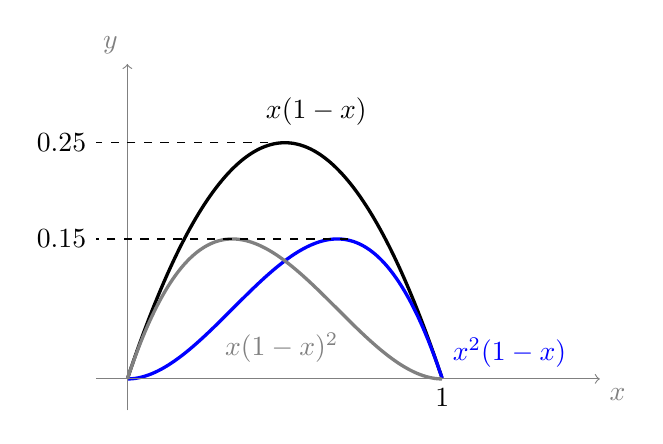
\begin{tikzpicture} [scale = 4]
	\draw[very thick, domain = 0:1, samples=200, smooth] plot (\x, {3*\x*(1-\x)});
	\draw[very thick, blue, domain = 0:1, samples=200, smooth] plot (\x, {3*\x*\x*(1-\x)}) node [above right] {$x^2(1-x)$};
	\draw[very thick, gray, domain = 0:1, samples=200, smooth] plot (\x, {3*\x*(1-\x)*(1-\x)});
	\draw [gray] (0.49,0.1) node {$\boldsymbol{x(1-x)^2}$};
	\draw [very thick] (0.6,0.85) node {$x(1-x)$};
	\draw [gray, ->] (0,-0.1) -- (0,1) node [above left] {$y$};
	\draw [gray, ->] (-0.1,0) -- (1.5,0) node [below right] {$x$};
	%\draw (3,2) node {Polynomials: $x,x^2,x^3$.};
	%\node [fill = white] at (pi,1.2) {$f(x) = x^m$};
	\draw (1,0) node [below] {$1$};
	\draw [dashed] (0.5,{3*0.5*(1-0.5)}) -- (-0.1,{3*0.5*(1-0.5)}) node [left] {$0.25$};
	\draw [dashed] (0.7,{3*0.33*(1-0.33)*(1-0.33)}) -- (-0.1,{3*0.33*(1-0.33)*(1-0.33)}) node [left] {$0.15$};
	\end{tikzpicture}
\end{center}
Notice that, for all $x \in [0,1],$ the $y$ values also remain between $0$ and $1$.
%NEED SOME WAY TO REFER BACK TO THIS EXAMPLE WHEN IT COMES IN HANDY LATER.


\subsection{Rational functions [$y = \frac{p(x)}{q(x)}$]} \label{rational}
The term ``rational'' is built out of the term ``ratio.'' So, just as rational numbers are \textit{numbers} that can be expressed as fractions of \textit{integers}, rational functions are \textit{functions} which can be expressed fractions of \textit{polynomials}. You can sort of think of polynomials as the integers of the realm of functions. Examples of rational functions include,
\[
f(x) = \frac{1}{x}, \qquad g(x) = \frac{1}{x^2}, \qquad k(x) = \frac{x^2}{1+x}.
\]
Some less obvious examples are,
\[
h(x) = x, \qquad q(x) = x^{-1}, \qquad p(x) = 1.
\]
Why is $h(x)$ a rational function? Well, because it can be \textbf{expressed as a fraction,} that is, \textit{it satisfies the definition of a rational function.} Technically, for a function to be rational we require that the numerator and denominator are polynomials. We can express $h(x)$ as
\[
h(x) = \frac{x}{1}.
\]
The numerator, $x$, and the denominator, $1$, are both polynomials, so $h(x)$ is a rational function. Similarly, we can rewrite $p(x)$ as,
\[
p(x) = \frac{1}{1}.
\]
The numerator and denominator of $p(x)$ are both polynomials, so $p(x)$ is a rational function. Finally, recalling index law (I4), we can rewrite $q(x)$ as
\[
q(x) = \frac{1}{x} \tag{since $x^{-1} = \frac{1}{x}$}
\]
Hence $q(x)$ is also a rational function. \\

\subsubsection{Some discontinuous functions}
Rational functions are a great place to look for discontinuous functions, because whenever we divide by a variable, $x$, the division will be undefined where $x = 0$. Consider the following (discontinuous) graph of $f(x) = \frac{1}{x}:$
\begin{center}
	\begin{tikzpicture} [scale = 1]
	\draw[very thick, domain = 0.3:3, samples=200, smooth] plot (\x, {1/\x});
	\draw[very thick, domain = -3:-0.3, samples=200, smooth] plot (\x, {1/\x});
	\draw [gray, ->] (0,-2.4) -- (0,3) node [above left] {$y$};
	\draw [gray, ->] (-2.5,0) -- (2.5,0) node [below right] {$x$};
	\draw (3,2) node {Graph of $f(x) = \frac{1}{x}$};
        \draw [fill = black] (0,0) circle (0.05cm) node [below left] {$(0,0)$};
	%\node [fill = white] at (pi,1.2) {$f(x) = x^m$};
	\end{tikzpicture}
\end{center}
Notice that the graph is in two pieces; one piece is to the left of the origin and one is to the right. Near the $y$-axis, each piece of the graph diverges away in the positive or negative direction (it diverges either upwards or downwards as $x$ gets closer to zero).  As $x$ gets closer to $0$, the graph will continue to get infinitely closer to the $y$-axis; however, the graph will never touch the $y$-axis, because $f(0)$ is undefined. This divergence is sometimes referred to as ``\textbf{asymptotic behaviour}.'' The $y$-axis is, in this case, referred to as the graph's ``\textbf{asymptote.}'' \\

\noindent Now, consider the graph of $k(x) = \frac{x^2}{1+x}$:
\begin{center}
	\begin{tikzpicture} [yscale = 0.5, scale = 0.7]
	\draw[very thick, domain = -0.83:3, samples=200, smooth] plot (\x, {\x*\x/(1 + \x)});
	\draw[very thick, domain = -3:-1.2, samples=200, smooth] plot (\x, {\x*\x/(1 + \x)});
	\draw [gray, ->] (0,-7) -- (0,3.5) node [above left] {$y$};
	\draw [gray, ->] (-3.5,0) -- (3.5,0) node [below right] {$x$};
	\draw (6.5,2) node {Graph of $\displaystyle{k(x) = \frac{x^2}{1+x}}$};
	%\node [fill = white] at (pi,1.2) {$f(x) = x^m$};
	\draw [dashed] (-1,-7) -- (-1,3.5);
	\draw (-1,0) node [below left] {$-1$};
	\end{tikzpicture}
\end{center}
This graph also has asymptotic behaviour, and is in two pieces. Hence this graph is also discontinuous. This time, the asymptote is the line parallel to the $y$-axis, passing through the point $x = -1$.
 The reason that this line is the asymptote is that when $x = -1$, the expression $1 + x$ becomes $1 - 1 = 0$, so the denominator of $k(x)$ is 0 when $x = -1$. Hence $k(x)$ is undefined at $x = -1$, which causes the asymptotic behaviour. \\
 
\noindent Now consider the graph of $g(x) = \frac{1}{x^2}:$
\begin{center}
	\begin{tikzpicture} [scale = 1]
	\draw[very thick, domain = 0.5:3, samples=200, smooth] plot (\x, {1/(\x*\x)});
	\draw[very thick, domain = -3:-0.5, samples=200, smooth] plot (\x, {1/(\x*\x)});
	\draw [gray, ->] (0,-2.4) -- (0,4.5) node [above left] {$y$};
	\draw [gray, ->] (-3.2,0) -- (3.2,0) node [below right] {$x$};
	\draw (3,2) node {Graph of $g(x) = \frac{1}{x^2}$};
        \draw [fill = black] (0,0) circle (0.05cm) node [below left] {$(0,0)$};
	%\node [fill = white] at (pi,1.2) {$f(x) = x^m$};
	\end{tikzpicture}
\end{center}
This graph is also in two pieces (so it is discontinuous), like the others, and it also exhibits asymptotic behaviour (the $y$-axis is its asymptote). Notce that, unlike the previous two graphs, this graph is actually symmetric about the $y$-axis (it is ``mirrored'' across the $y$-axis). This symmetry arises from the fact that $x^2$ has the same sign when $x$ is positive as it does when $x$ is negative; i.e., $x^2 = (-x)^2,$ because squaring a negative number gives a positive number. \label{symmetric function} \label{mirrored} \\

\subsubsection{Using rational functions as probability measures}
\noindent Have a look again at the three graphs of $f(x), k(x),$ and $g(x)$; try to decide what happens in each case as $x$ gets infinitely large in the positive direction (to the right, i.e., as $x \rightarrow \infty$) and as $x$ gets infinitely large in the negative direction (to the left, i.e., as $x \rightarrow -\infty$).
\begin{center}
	\begin{tikzpicture} [scale = 1]
	%\draw[very thick, domain = 0.3:3, samples=200, smooth] plot (\x, {1/\x});
	%\draw[very thick, domain = -3:-0.3, samples=200, smooth] plot (\x, {1/\x});
	\draw [gray, ->] (0,-2.4) -- (0,3) node [above left] {$y$};
	\draw [gray, ->] (-4.5,0) -- (4.5,0) node [below right] {$x$};
	%\draw (3,2) node {Graph of $f(x) = \frac{1}{x}$};
	\draw (3,-0.3) node {$x \longrightarrow \infty$};
	\draw (-3,-0.3) node {$-\infty \longleftarrow x$};
        \draw [fill = black] (0,0) circle (0.05cm) node [below left] {$(0,0)$};
	%\node [fill = white] at (pi,1.2) {$f(x) = x^m$};
	\end{tikzpicture}
\end{center}

\noindent You should be able to tell from the graphs that $f(x)$ and $g(x)$ both approach zero as $x \rightarrow \infty$ and as $x \rightarrow -\infty$. This makes sense because, as $x$ and $x^2$ get infinitely large, the expressions $\frac{1}{x}$ and $\frac{1}{x^2}$ get infinitely small. \\

\noindent However, you should also notice that the function $k(x)$ does not approach zero as $x$ gets infinitely large in either direction. Instead, $k(x)$ heads towards the $x$-axis (even touching the $x$-axis at $x = 0$) then takes a turn and starts heading away from the $x$-axis as $x$ increases in size. This too makes sense when we consider that the expression $\frac{x^2}{1+x}$ has $x^2$ in the numerator, and only $1+x$ in the denominator; so, as $x$ gets large the numerator will grow faster than the denominator, and thus $k(x)$ will keep getting further from $0$. \\

\noindent The behaviours of functions on a given domain are of interest to us because probabilities are values between $0$ and $1$. That is, for a function $p(x)$ to be useful as a probability measure, we require that $0 \leq p(x) \leq 1$ for all values of $x$ in the domain of $p(x)$; for the functions $f(x) = \frac{1}{x}$ and $g(x) = \frac{1}{x^2}$, this is true whenever $x \geq 1$:

\begin{center}
\begin{minipage}{0.4\textwidth}
	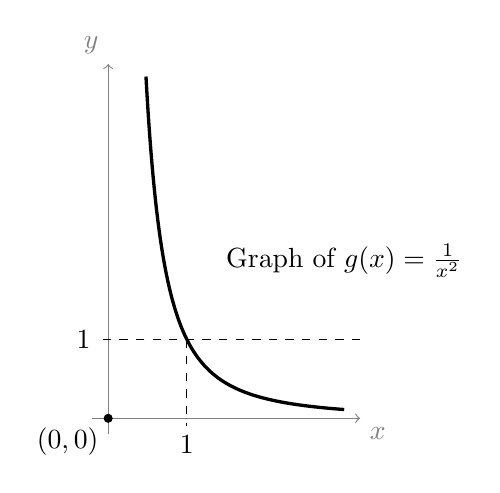
\begin{tikzpicture} [scale = 1]
	\draw[very thick, domain = 0.48:3, samples=200, smooth] plot (\x, {1/(\x*\x)});
	%\draw[very thick, domain = -3:-0.5, samples=200, smooth] plot (\x, {1/(\x*\x)});
	\draw [gray, ->] (0,-0.2) -- (0,4.5) node [above left] {$y$};
	\draw [gray, ->] (-0.2,0) -- (3.2,0) node [below right] {$x$};
	\draw (3,2) node {Graph of $g(x) = \frac{1}{x^2}$};
        \draw [fill = black] (0,0) circle (0.05cm) node [below left] {$(0,0)$};
        \draw [dashed] (3.2,1) -- (-0.1,1) node [left] {$1$};
        \draw [dashed] (1,1) -- (1,-0.1) node [below] {$1$};
	%\node [fill = white] at (pi,1.2) {$f(x) = x^m$};
	\end{tikzpicture}
\end{minipage}%
\begin{minipage}{0.4\textwidth}
	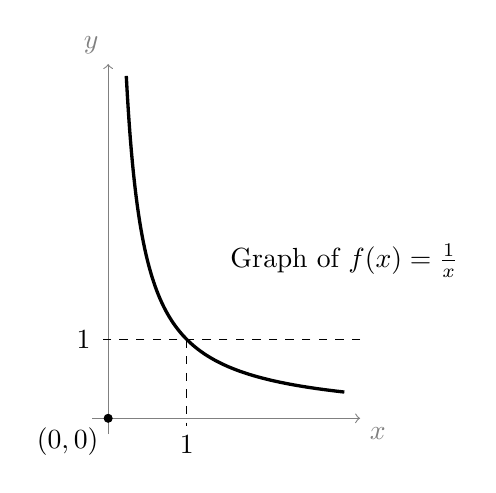
\begin{tikzpicture} [scale = 1]
	\draw[very thick, domain = 0.23:3, samples=200, smooth] plot (\x, {1/\x});
	%\draw[very thick, domain = -3:-0.3, samples=200, smooth] plot (\x, {1/\x});
	\draw [gray, ->] (0,-0.2) -- (0,4.5) node [above left] {$y$};
	\draw [gray, ->] (-0.2,0) -- (3.2,0) node [below right] {$x$};
	\draw (3,2) node {Graph of $f(x) = \frac{1}{x}$};
        \draw [fill = black] (0,0) circle (0.05cm) node [below left] {$(0,0)$};
	%\node [fill = white] at (pi,1.2) {$f(x) = x^m$};
	\draw [dashed] (3.2,1) -- (-0.1,1) node [left] {$1$};
        \draw [dashed] (1,1) -- (1,-0.1) node [below] {$1$};
	\end{tikzpicture}
\end{minipage}
\end{center}
Hence $f(x)$ and $g(x)$ could be useful as probability measures, as long as we restrict the domain to the interval $x \geq 1$. 

\subsection{Powers (non-integer)  [$y = x^\frac{1}{n}$]} \label{powers (non-integer)}
In section \ref{fractional indices}, we showed that for real numbers $x,y$ with $x \geq 0$, and for some natural number $n$, the equation
\[
y^n = x
\]
has the solution
\[
y = x^\frac{1}{n}.
\]
This leads us to deal with functions of the form $f(x) = x^\frac{1}{n}$ (or, if you like, $f(x) = \sqrt[n]{x}$). Of particular interest to us (doing probability), is the behaviour of these functions near $x = 1$. Below are overlayed graphs of $f(x) = x^\frac{1}{n}$, for $n = 1,2$ and $3:$
%\begin{center}
%	\begin{tikzpicture} [scale = 1.3]
%%	\begin{axis}[smooth,enlargelimits=false,xmin=-0.2,xmax=3,ymin=-0.2,ymax=2.4,axis x line=bottom,axis y line=left]
%%	   %\addplot[very thick, domain=-0.1:3,samples=200] {(x)};
%%	   \addplot[very thick, blue, domain=-1:3,samples=200, unbounded coords = jump] {(x)^(1/2)};
%%            %\addplot[thick, gray, domain=0:3] {(x/abs(x)*(abs(x))^(1/3)};
%%            %\addplot[thin,dotted] coordinates {(1,0) (1,1)};
%%            %\addplot[thin,dotted] coordinates {(0,1) (1,1)};
%%        \end{axis}
%	\begin{axis}[hide axis]
%       \addplot[very thick, domain=0:3,samples=200] {(x)} node [above right] {$x$};
%       \addplot[very thick, gray,domain=0:3, samples=200]{x/abs(x)*abs(x)^(1/3)} node [above right] {$x^\frac{1}{3}$};
%       \addplot[very thick, blue, domain=0:3,samples=200] {(x)^(1/2)} node [above right] {$x^\frac{1}{2}$};
%       \end{axis}
%        \draw [gray, ->] (0+0.55,-0.1) -- (0+0.55,5.5) node [above left] {$y$};
%	\draw [gray, ->] (-0.1,0+0.45) -- (6,0+0.45) node [below right] {$x$};
%	\draw [dashed] (2.5,2.1) -- (2.5,0.3) node [below] {$1$};
%	\draw [dashed] (2.5,2.1) -- (0.3,2.1) node [left] {$1$};
%	\end{tikzpicture}
%\end{center}
\begin{center}
	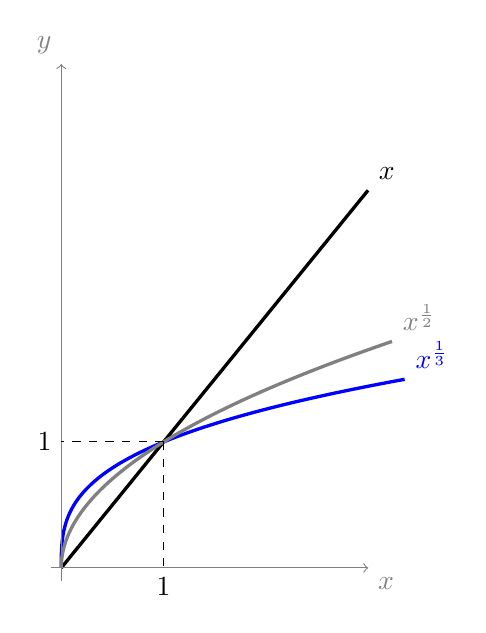
\begin{tikzpicture} [yscale = 1.6,xscale = 1.3]
%	\begin{axis}[smooth,enlargelimits=false,xmin=-0.2,xmax=3,ymin=-0.2,ymax=2.4,axis x line=bottom,axis y line=left]
%	   %\addplot[very thick, domain=-0.1:3,samples=200] {(x)};
%	   \addplot[very thick, blue, domain=-1:3,samples=200, unbounded coords = jump] {(x)^(1/2)};
%            %\addplot[thick, gray, domain=0:3] {(x/abs(x)*(abs(x))^(1/3)};
%            %\addplot[thin,dotted] coordinates {(1,0) (1,1)};
%            %\addplot[thin,dotted] coordinates {(0,1) (1,1)};
%        \end{axis}
	\draw[very thick, domain = 0:3, samples=200, smooth] plot (\x,\x) node [above right] {$x$};
	\draw[very thick, blue, domain = 0:1.5, samples=200, smooth] plot ({(\x)^3},\x) node [above right] {$x^\frac{1}{3}$};
	\draw[very thick, gray, domain = 0:1.8, samples=200, smooth] plot ({(\x)^2},\x) node [above right] {$x^\frac{1}{2}$};
        \draw [gray, ->] (0,-0.1) -- (0,4) node [above left] {$y$};
	\draw [gray, ->] (-0.1,0) -- (3,0) node [below right] {$x$};
	\draw [dashed] (1,1) -- (1,0) node [below] {$1$};
	\draw [dashed] (1,1) -- (0,1) node [left] {$1$};
	\end{tikzpicture}
\end{center}
One important observation is that when $0 \leq x \leq 1$ the value of $f(x) = x^\frac{1}{n}$ is \textit{greater} for greater values of $n$. Contrast this with the graphs of $h(x) = x^m$, for $m = 1,2$ and $3$, from section \ref{polynomials}. \\

\noindent Also, notably, on the interval $x \in [0,1]$, the values of $f(x) = x^\frac{1}{n}$ always lie between 0 and 1. When $x > 1$, on the other hand, we get $f(x) > 1$. Finally, for $x < 0$, the values of $f(x)$ are either negative or undefined. This implies that functions of the form $f(x)$ make useful probability measures only when their domain is restricted to the interval $x \in [0,1].$


\subsection{Exponentials [$y = b^x$]} \label{exponentials}
We have seen power functions, $f(x)$, where $f(x) = x^b$; the base is a variable, and the index, $b$, is a constant. Now, let's have a look at functions of the form
\[
k(x) = b^x, \qquad \text{with $b > 0.$}
\]   
This time, the constant, $b$, is the base, and the index is the variable, $x$. These are not power functions; these are called \textbf{exponential functions.} \\ \label{exponential function 2}

\noindent One particular exponential function is so ubiquitous, and so important, that it is called \textit{the} \textbf{Exponential function} (with a capitol ``E''). This is the exponential function with base $b = \e$, which was introduced in section \ref{sec4012} on page \pageref{sec4012}. Sometimes this function is written $\text{exp}(x)$, so that \label{symbexp(x)}

	\bigskip
	
	\hfil\fbox{
	\begin{minipage}{0.23\columnwidth}{
	
	\vskip 0.03cm
	\begin{center}
	$\text{exp}(x) = \e^x.$
	\end{center}
	}
	\end{minipage}}
	\bigskip
	
\noindent Below are graphs of the functions $k(x) = 2^x$, $\text{exp}(x)$, and $q(x) = 4^x$.  
\begin{center}
	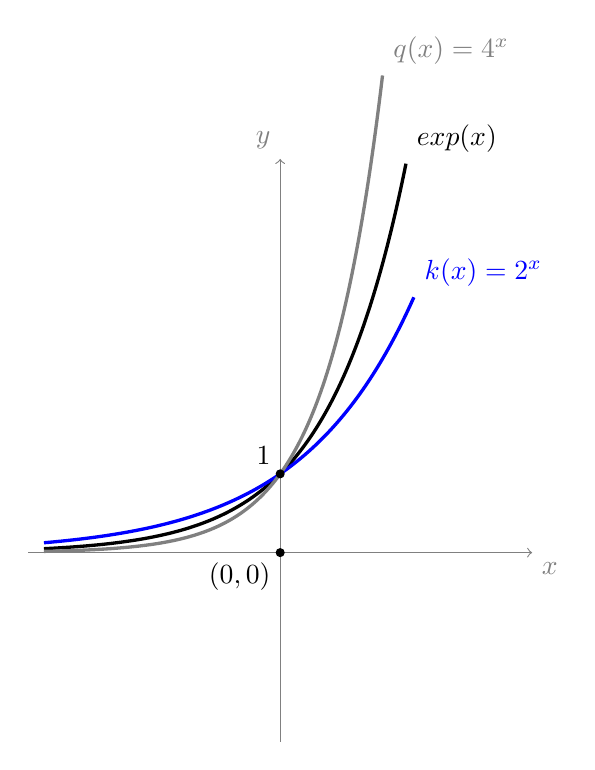
\begin{tikzpicture} [scale = 1]
	\draw[very thick, domain = -3:1.6, samples=200, smooth] plot (\x,{exp(\x)}) node [above right] {$\text{exp}(x)$};
	\draw[very thick, blue, domain = -3:1.7, samples=200, smooth] plot (\x,{exp(ln(2)*\x)}) node [above right] {$k(x) = 2^x$};
	\draw[very thick, gray, domain = -3:1.3, samples=200, smooth] plot (\x,{exp(ln(4)*\x)}) node [above right] {$q(x) = 4^x$};
	\draw [gray, ->] (0,-2.4) -- (0,5) node [above left] {$y$};
	\draw [gray, ->] (-3.2,0) -- (3.2,0) node [below right] {$x$};
	%\draw (3,2) node {Graph of $g(x) = \e^x$};
        \draw [fill = black] (0,0) circle (0.05cm) node [below left] {$(0,0)$};
	%\node [fill = white] at (pi,1.2) {$f(x) = x^m$};
	\draw (0,1) [fill = black] circle (0.05cm) node [above left] {$1$};
	\end{tikzpicture}
\end{center}
Notice that all three graphs pass through the point $(0,1)$; and when $x < 0$, the outputs are between $0$ and $1$. These properties hold for $b^x$ whenever $b$ is greater than $1$. Also, for all $x$, the outputs are positive; this is true for all $b > 0$. \\

\noindent Furthermore, it is true that any exponential function, with base $b$ where $b > 1$, will have the property that $b^x \rightarrow \infty$ as $x \rightarrow \infty$, and that $b^x \rightarrow 0$ as $x \rightarrow -\infty$. \\

\noindent What about the function $e^{-x}$? This function will be very similar to $e^x$, except wherever $x$ is positive, $-x$ will be negative, and wherever $x$ is negative $-x$ will be positive. This has the effect of ``flipping'' the $x$-axis coordinates across the $y$-axis, as follows:
\begin{center}
	\begin{tikzpicture} [scale = 1]
	\draw[very thick, domain = -1.4:3, samples=200, smooth] plot (\x,{exp(-\x)}) node [above right] {$\text{exp}(-x)$};
	\draw [gray, ->] (0,-2.4) -- (0,3.2) node [above left] {$y$};
	\draw [gray, ->] (-4.5,0) -- (4.5,0) node [below right] {$x$};
	\draw (2.8,-0.4) node {$(-x) \longrightarrow -\infty$};
	\draw (-2.8,-0.4) node {$\infty \longleftarrow (-x)$};
	%\draw (3,2) node {Graph of $g(x) = \e^x$};
        %%\draw [fill = black] (0,0) circle (0.05cm) node [below left] {$(0,0)$};
	%\node [fill = white] at (pi,1.2) {$f(x) = x^m$};
	%%\draw (0,1) [fill = black] circle (0.05cm) node [above left] {$1$};
	\end{tikzpicture}
\end{center}
So, the graph of $\text{exp}(-x)$ is just like the graph of $\text{exp}(x)$, but it is flipped across the $y$-axis:
\begin{center}
	\begin{tikzpicture} [scale = 1]
	\draw[very thick, domain = -1.6:3, samples=200, smooth] plot (\x,{exp(-\x)}) node [above right] {$\text{exp}(-x)$};
	\draw[very thick, blue, domain = -3:1.6, samples=200, smooth] plot (\x,{exp(\x)}) node [above right] {$\text{exp}(x)$};
	\draw [gray, ->] (0,-2.4) -- (0,5) node [above left] {$y$};
	\draw [gray, ->] (-3.2,0) -- (3.2,0) node [below right] {$x$};
	%\draw (3,2) node {Graph of $g(x) = \e^x$};
        \draw [fill = black] (0,0) circle (0.05cm) node [below left] {$(0,0)$};
	%\node [fill = white] at (pi,1.2) {$f(x) = x^m$};
	\draw (0,1) [fill = black] circle (0.05cm) node [right] {$1$};
	\end{tikzpicture}
\end{center}
The function $e^{-x}$, with a positive domain, could be useful to us as a probability measure; the output of $e^{-x}$ remains between $0$ and $1$ for all $x \geq 0$.

\section{Logarithms [$y = \log_b(x)$]} \label{symblog}
Suppose that we wish to solve the following equation to find $y$, where $b > 0,$
\[
x = b^y
\]
This equation involves exponentiation of the base $b$, by the variable $y$, on the right hand side. \\

\noindent In section \ref{powers (non-integer)} we solved $y^n = x$ by raising both sides to the power of $\frac{1}{n}$, which cancelled with the power $n$, leaving just $y$ on the left hand side; we saw that raising an expression to the power $\frac{1}{n}$ ``undoes'' the effect of raising it to the power of $n$. For this reason, raising to the power of $n$ and raising to the power of $\frac{1}{n}$ are called \textbf{inverse} operations. \label{inverse operations.} \\

\noindent In order to solve the equation $x = b^y$, we will need a function which is \textit{inverse} to the exponential function. \\

\noindent Luckily, this function already exists; it is called the \textbf{logarithm.} \\

\noindent The logarithm is the function that ``undoes'' exponentiation. In other words, the logarithm of a number, $x$, is the exponent, $y$, to which the base, $b$, must be raised to produce $x$. We write $y = \log_b(x)$. \\

\noindent The definition of a logarithm can seem a bit confusing at first, but once it clicks it makes perfect sense, so, we will go over it again, keeping in mind that it is really just \textit{defined} as the inverse to exponentiation: If we write $y = \log_b(x)$, then this means that $b^y = x$. In other words, if I asked you, ``hey, what number, $y$, do I have to raise $b$ to, in order to get $x$?'' Then you would tell me, ``the answer is $y = \log_b(x)$.'' \\

\noindent Put very simply: 

	\bigskip
	
	\hfil\fbox{
	\begin{minipage}{0.33\columnwidth}{
	
	\vskip 0.03cm
	\begin{center}
	$b^y = x \iff y = \log_b(x)$
	\end{center}
	}
	\end{minipage}}
	\bigskip
	
\noindent The symbol $\iff$ means ``is equivalent to.'' \label{symbiff} \\

\noindent We read $\log_b(x)$ as ``log base $b$ of $x$.'' When we leave out the $b$ and write $\log(x)$ this conventionally means $\log_{10}(x)$, that is, leaving out the $b$ implies $b = 10$. Since the Exponential function, $\e^x$, gets its own symbol, $\text{exp}(x)$, it is only fair that $\log_e(x)$ gets its own symbol as well; we write ``$\ln(x)$'' and say ``natural logarithm of $x$'' to mean ``$\log_\e(x)$.'' NOTE: Dont get \textit{the} Exponential function (that with base $\e$) confused with exponential functions in general (those with base $b$); the inverse of an exponential function with base $b$ is the logarithm with base $b$. \\

\noindent \textbf{Two of the most important properties of logarithms are:} \label{log2properties} \label{symbln} \\

	\bigskip
	
	\hfil\fbox{
	\begin{minipage}{0.7\columnwidth}{
	
	\vskip 0.04cm
	\begin{center}
	(i) \;\; $b^{\log_b(x)} = x,$ \qquad and \qquad (ii) \;\; $\log_b(b^x) = x$.
	\end{center}
	}
	\end{minipage}}
	\bigskip
	\bigskip
	
\noindent The interpretation of property (i) in words is a tongue twister: ``$x$ is the number that we get when we raise $b$ to the power of the number that we raise $b$ to in order to get~$x$.'' \\

\noindent Interpreting property (ii) in words we can say: ``$x$ is the power that we raise $b$ to in order to get $b^x$.'' \\

\noindent If you read them a couple of times, you should realise that the only reason why the two sentences above sound strange is that they are \textit{stating the obvious} (and perhaps that they are worded badly). In fact, properties (i) and (ii) are just another way of capturing the definition of a logarithm. \\

\noindent We will use properties (i) and (ii) to help us simplify and rearrange expressions involving logarithms; but before we get onto some examples, let's have a look at their graphs.

\subsection{Graphing logarithms}

\noindent When graphing logarithms, we will need to consider a couple of important facts: Recall (from section \ref{exponentials}) that exponential functions always give positive outputs. Hence, the function $f(x) = \log_b(x)$ only makes sense when $x > 0$. Furthermore, since the exponential function has all real numbers in its domain, we should expect the \textit{outputs} of $\log_b(x)$ to be all real numbers. \\

\noindent The answer to the following question will also be useful when graphing logarithms (try to answer it yourself before seeing the solution): \\
\noindent \textbf{Question: For all $b > 0$, what is $\boldsymbol{\log_b(1)?}$} \\ \\

\noindent \textit{Solution:} \\
\noindent If we rephrase the question, it is asking: ``\textbf{What power, $\boldsymbol{y}$, should I raise $\boldsymbol{b}$ to in order to get $\boldsymbol{b^y = 1}$?}'' The answer is, of course, $y = 0$, because $b^0 = 1$ for all $b > 0$. Hence

	\bigskip
	
	\hfil\fbox{
	\begin{minipage}{0.3\columnwidth}{
	
	\vskip 0.04cm
	\begin{center}
	$\log_b(1) = 0,$ \\
	for all $b > 0$. 
	\end{center}
	}
	\end{minipage}}
	\bigskip
	\bigskip
	
\noindent Below are the graphs of $f(x) = \log_{10}(x), g(x) = \log_\e(x)$ and $k(x) = \log_2(x)$:
\begin{center}
	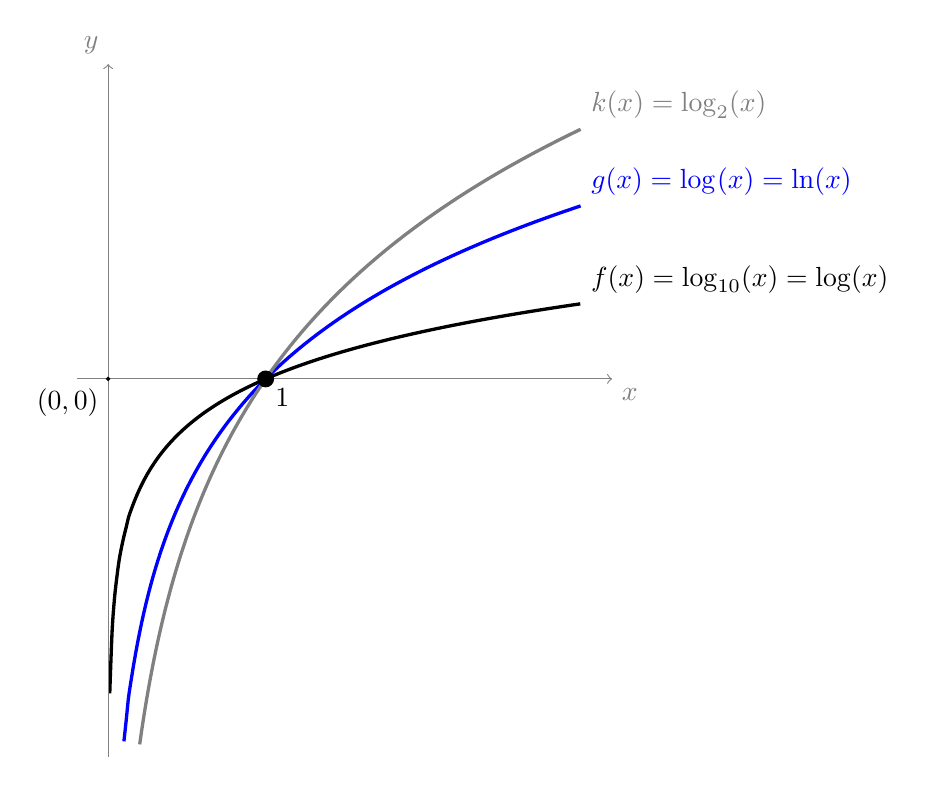
\begin{tikzpicture} [scale = 2]
	\draw[very thick, domain = 0.01:3, samples=200, smooth] plot (\x,{ln(\x)/ln(10)}) node [above right] {$f(x) = \log_{10}(x) = \log(x)$};
	\draw[very thick, blue, domain = 0.1:3, samples=200, smooth] plot (\x,{ln(\x)}) node [above right] {$g(x) = \log_{\e}(x) = \ln(x)$};
	\draw[very thick, gray, domain = 0.2:3, samples=200, smooth] plot (\x,{ln(\x)/ln(2)}) node [above right] {$k(x) = \log_{2}(x)$};
	\draw [gray, ->] (0,-2.4) -- (0,2) node [above left] {$y$};
	\draw [gray, ->] (-0.2,0) -- (3.2,0) node [below right] {$x$};
	%\draw (3,2) node {Graph of $g(x) = \e^x$};
        \draw [fill = black] (0,0) circle (0.01cm) node [below left] {$(0,0)$};
	%\node [fill = white] at (pi,1.2) {$f(x) = x^m$};
	\draw (1,0) [fill = black] circle (0.05cm) node [below right] {$1$};
	\end{tikzpicture}
\end{center}
Notice that all three graphs pass through the point $(1,0)$; this is because $\log_b(1) = 0$ for all $b > 0$. Also, notice that all three graphs have the $y$-axis as an asymptote; the graph of a logarithm will never touch the $y$-axis, because

	\bigskip
	
	\hfil\fbox{
	\begin{minipage}{0.4\columnwidth}{
	
	\vskip 0.04cm
	\begin{center}
	$\log_b(0)$ is undefined.
	\end{center}
	}
	\end{minipage}}
	\bigskip
	
\noindent Why is $\log_b(0)$ undefined? The reason is that there is no power, $y$, that you can raise~$b$ to in order to get $b^y = 0$. In other words, $0$ is not an output of the exponential function, so, $0$ cannot be an input of the logarithm function.

\subsection{Logarithm laws} \label{log laws}
The following four laws will be very useful to us while working with logarithms:
\begin{itemize}
\item $\log_b(x) + \log_b(y) = \log_b(xy)$ \hfill (L1)
\item $\log_b(x^p) = p\log_b(x)$ \hfill (L2)
\item $\log_b(1) = 0$ \hfill  (L3)
\item $\log_b\brac{\frac{1}{x}} = -\log_b(x)$ \hfill  (L4)
\end{itemize}
Each can be derived from the index laws: (L1) is based on index law (I1); (L2) is based on (I2); (L3) is based on (I3); and (L4) is based on (I4).

\subsubsection{Proof that the logarithm laws follow from the index laws}
In each case it is necessary to remember properties (i) and (ii) from section \ref{log2properties} on~page~\pageref{log2properties}. In all of the following proofs we start with something obvious then show. using index laws, that this leads to the required logarithm law. \\


\noindent \textbf{(L1) follows from (I1):} \\
Let $b,x,y > 0$. It is obvious that
\[
xy = xy.
\] 
Using property (i) of logarithms, this is equivalent to
\[
b^{\log_b(x)}b^{\log_b(y)} = xy.
\]
Using index law (I1) on the left hand side gives
\[
b^{\log_b(x) + \log_b(y)} = xy.
\]
Taking the logarithm, base $b$, of both sides, then using property (ii) on the left hand side gives
\[
\log_b(x) + \log_b(y) = \log_b(xy).
\]
\bigskip

\noindent \textbf{(L2) follows from (I2):} \\
Let $b,x,y > 0$ and let $p \in \R$. It is obvious that
\[
x^p = x^p.
\]
Using property (i) on the right hand side gives
\[
x^p = \brac{b^{\log_b(x)}}^p.
\]
Using index law (I2) we get
\[
x^p = b^{p\log_b(x)}.
\]
Taking logarithm, base $b$, of both sides, then using property (ii) on the right hand side,
\[
\log_b(x^p) = p\log_b(x).
\]
\bigskip

\noindent \textbf{(L3) follows from (I3):} \\
Let $b > 0$. Index law (I3) states that
\[
1 = b^0.
\]
Taking the logarithm, base $b$, of both sides, we get
\[
\log_b(1) = \log_b(b^0).
\]
Using property (ii) on the right hand side gives
\[
\log_b(1) = 0.
\]
\bigskip

\noindent \textbf{(L4) follows from (I4):} \\
Let $x,b > 0$. It is obvious that
\[
\frac{1}{x} = \frac{1}{x}.
\]
Using property (i) on the right hand side gives
\[
\frac{1}{x} = \frac{1}{b^{\log_b(x)}}.
\]
Using index law (I4) on the right hand side gives
\[
\frac{1}{x} = b^{-\log_b(x)}.
\]
Taking logarithm, base $b$, of both sides, then using property (ii) on the right hand side,
\[
\log_b\brac{\frac{1}{x}} = -\log_b(x).
\]
\bigskip

\noindent Hence the logarithm laws follow from the index laws, as required.

\subsection{Example}
Let $x > 0$. Solve for $x$ in the equation
\[
2\log(x) + \log(4) = 6.
\]
Recall that ``$\log(x)$'' means: Logarithm, base 10, of $x$. \\ \\



\noindent \textit{Solution:} \\

\noindent Using law (L2) gives,
\[
\log(x^2) + \log(4) = 6.
\]
Using law (L1) gives,
\[
\log(4x^2) = 6.
\]
Making both sides into powers of 10,
\[
10^{\log(4x^2)} = 10^6.
\]
Using logarithm property (i) (i.e., $b^{\log_b(x)} = x$) on the left hand side,
\[
4x^2 = 10^6.
\]
Dividing both sides by $4$,
\[
x^2 = \frac{10^6}{4}.
\]
Raising both sides to the power of $\frac{1}{2}$,
\[
\brac{x^2}^\frac{1}{2} = \bfrac{10^6}{4}^\frac{1}{2}.
\]
Using index law (I2) gives,
\[
x^\frac{2}{2} = \frac{10^\frac{6}{2}}{4^\frac{1}{2}}.
\]
Simplifying, and noting that $4^\frac{1}{2} = \sqrt{4} = 2$ we get,
\[
x = \frac{10^3}{2}.
\]
Since $10^3 = 1000$, this simplifies to
\[
x = \frac{1000}{2} = 500.
\]

\subsection{Examples:}
Try to do these before looking at the solutions. Solve for $x$:
\begin{enumerate}
\item $\ln(3 + x) = 4$
\item $\e^{x + 9} = 1$
\item $3\e^x = \e^{-x}$ 
\end{enumerate}
Recall that ``$\ln(x)$'' means ``logarithm, base $\e$, of $x$.''
\bigskip

\noindent \textit{Solution to (1):} \\
\begin{align*}
\ln(3 + x) = 4 & \iff e^{\ln(3 + x)} = \e^4 \tag{Making both sides powers of $\e$} \\
			& \iff 3 + x = \e^4 \tag{Using log property (i), page \pageref{log2properties}} \\
			& \iff x = \e^4 - 3. \tag{Subtracting 3 from both sides}
\end{align*}
\bigskip

\noindent \textit{Solution to (2):} \\
\begin{align*}
\e^{x + 9} = 1 & \iff \ln(e^{x + 9}) = \ln(1) \tag{taking natural log of both sides} \\
			& \iff x + 9 = \ln(1) \tag{Using log property (ii), page \pageref{log2properties}} \\
			& \iff x + 9 = 0 \tag{Using log law (L3)} \\
			& \iff x = -9. \tag{Subtracting 9 from both sides}
\end{align*}

\noindent \textit{Solution to (3):} \\
\begin{align*}
3\e^x = \e^{-x} & \iff 3\e^x\e^x = \e^x\e^{-x} \tag{Multiplying both sides by $\e^x$} \\
			   & \iff 3\e^{x + x} = \e^{x - x} \tag{Using index law (I1)} \\ \bigskip
			   & \iff 3\e^{2x} = \e^0 \tag{Simplifying} \\
			   & \iff 3\e^{2x} = 1 \tag{Using index law (I3)} \\
			   & \iff \e^{2x} = \frac{1}{3} \tag{Dividing both sides by $3$} \\
			   & \iff \ln\brac{\e^{2x}} = \ln\brac{\frac{1}{3}} \tag{Taking natural log of both sides} \\
			   & \iff 2x = \ln\brac{\frac{1}{3}} \tag{Using log property (ii), page \pageref{log2properties}} \\
			   & \iff 2x = -\ln(3) \tag{Using log law (L4)} \\
			   & \iff x = \frac{-\ln(3)}{2}. \tag{Dividing both sides by 2}
\end{align*}

\section{Gaussian curve (or Bell curve)} \label{gaussian curve} \label{bell curve}
One extremely important function in probability and statistics (and physcis, chemistry, biology,$\ldots$) is the function
\[
f(x) = \e^{-x^2}.
\]
This function is called a \textbf{Gaussian.} We will see an important application of the Gaussian in section \ref{normal distribution}. \\
%WOULD BE GOOD TO SAY WHICH LECTURE IT COMES UP IN!!!!


\noindent Let's try and predict what the graph of $f(x)$ will look like: One thing that we know for sure is that it will be symmetric about the $y$-axis; this is because the variable, $x$, is squared, so the output will be exactly the same for positive values of $x$ as it is for negative values of $x$. Another thing we know, from our knowledge of exponential functions (see section \ref{exponentials}), is that the output will decrease as $x$ gets larger in size (i.e., as we move further from the $y$-axis); this is because index law (I4) tells us that $\e^{-x^2} = \frac{1}{\e^{x^2}}$, which gets smaller as its denominator grows. So, $f(x)$ is symmetric, and it is decreasing as we get further from the $x$-axis; this must mean that the maximum output is when $x = 0$, i.e., the function will be tallest when it crosses the $y$-axis. \\

\noindent We can think of $f(x)$ as the composition of $\e^x$ with the function $-x^2$. Below is the graph of $f(x),$ along with $k(x) = \e^{-x}$ and $g(x) = -x^2$:
\begin{center}
	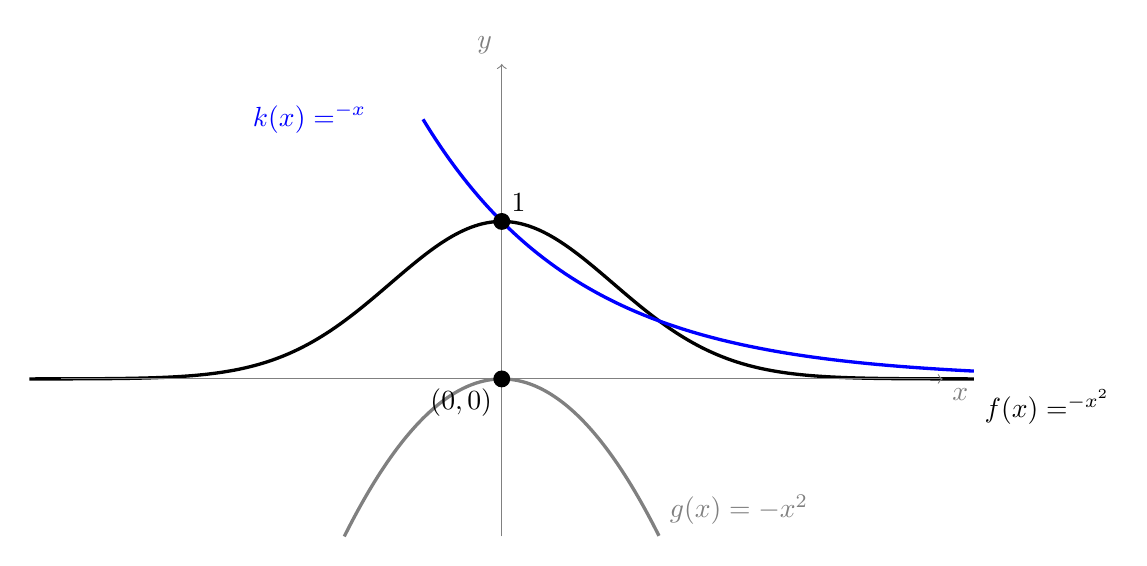
\begin{tikzpicture} [scale = 2]
	\draw[very thick, domain = -3:3, samples=200, smooth] plot (\x,{exp(-(\x)^2)}) node [below right] {$f(x) = \e^{-x^2}$};
	\draw[very thick, blue, domain = -0.5:3, samples=200, smooth] plot (\x,{exp(-(\x))});
	\draw [blue] (-0.8,1.5) node [above left] {$k(x) = \e^{-x}$};
	\draw[very thick, gray, domain = -1:1, samples=200, smooth] plot (\x,{-(\x)^2}) node [above right] {$\boldsymbol{g(x) = -x^2}$};
	\draw [gray, ->] (0,-1) -- (0,2) node [above left] {$y$};
	\draw [gray, ->] (-2.8,0) -- (2.8,0) node [below right] {$x$};
	%\draw (3,2) node {Graph of $g(x) = \e^x$};
        \draw [fill = black] (0,0) circle (0.05cm) node [below left] {$(0,0)$};
	%\node [fill = white] at (pi,1.2) {$f(x) = x^m$};
	\draw (0,1) [fill = black] circle (0.05cm) node [above right] {$1$};
	\end{tikzpicture}
\end{center}
Notice that the output, $f(x)$, never goes above $y = 1$ (this will be a useful feature if we want to use $f(x)$ as a probability measure). Also, as $x \rightarrow \pm\infty$ the Gaussian approaches $0$ faster than $\e^{-x}$.